\chapter{ผลการทดสอบแบตเตอรี่ตามมาตรฐาน}
ในบทนี้จะแสดงถึงการทดสอบแบตเตอรี่ตามมาตรฐานและทดสอบในหัวข้อต่างๆที่ได้กล่าวไว้ในบทที่ผ่านมาซึ่งผลที่ได้จากการทดสอบในแต่ละหัวข้อจะถูกอธิบายอย่างละเอียด
%==========================================================================================
\section{การทดสอบตามมาตรฐาน UN ECE R136}
ในหัวข้อการทดสอบนี้จะทดสอบแบตเตอรี่ด้วยกันทั้งสิ้น 3 โมดูลคือ
\begin{itemize}
 {\item แบตเตอรี่สำหรับจักรยานยนต์ไฟฟ้า 72V 30Ah}
 {\item แบตเตอรี่สำหรับรถสามล้อไฟฟ้า 72V 60Ah}
 {\item แบตเตอรี่ 72V 72Ah}
\end{itemize}
และทดสอบด้วยกันทั้ง 2 หัวข้อจาก 10 หัวข้อจากมาตรฐาน UN ECE R136 คือ
\begin{itemize}
 {\item การทดสอบการป้องกันการชาร์จเกิน}
 {\item การทดสอบการป้องกันการดิสชาร์จเกิน}
\end{itemize}
ซึ่งผลจากการทดสอบมีดังนี้
%-------------------------------------------
\pagebreak
\subsection{ผลการทดสอบการป้องกันการชาร์จเกิน}
สำหรับการทดสอบการป้องกันการชาร์จเกินของแบตเตอรี่สำหรับจักรยานยนต์ไฟฟ้า 72V 30Ah มีดังนี้
\begin{center}
	\begin{figure}[H]
	\makebox[\textwidth]{
	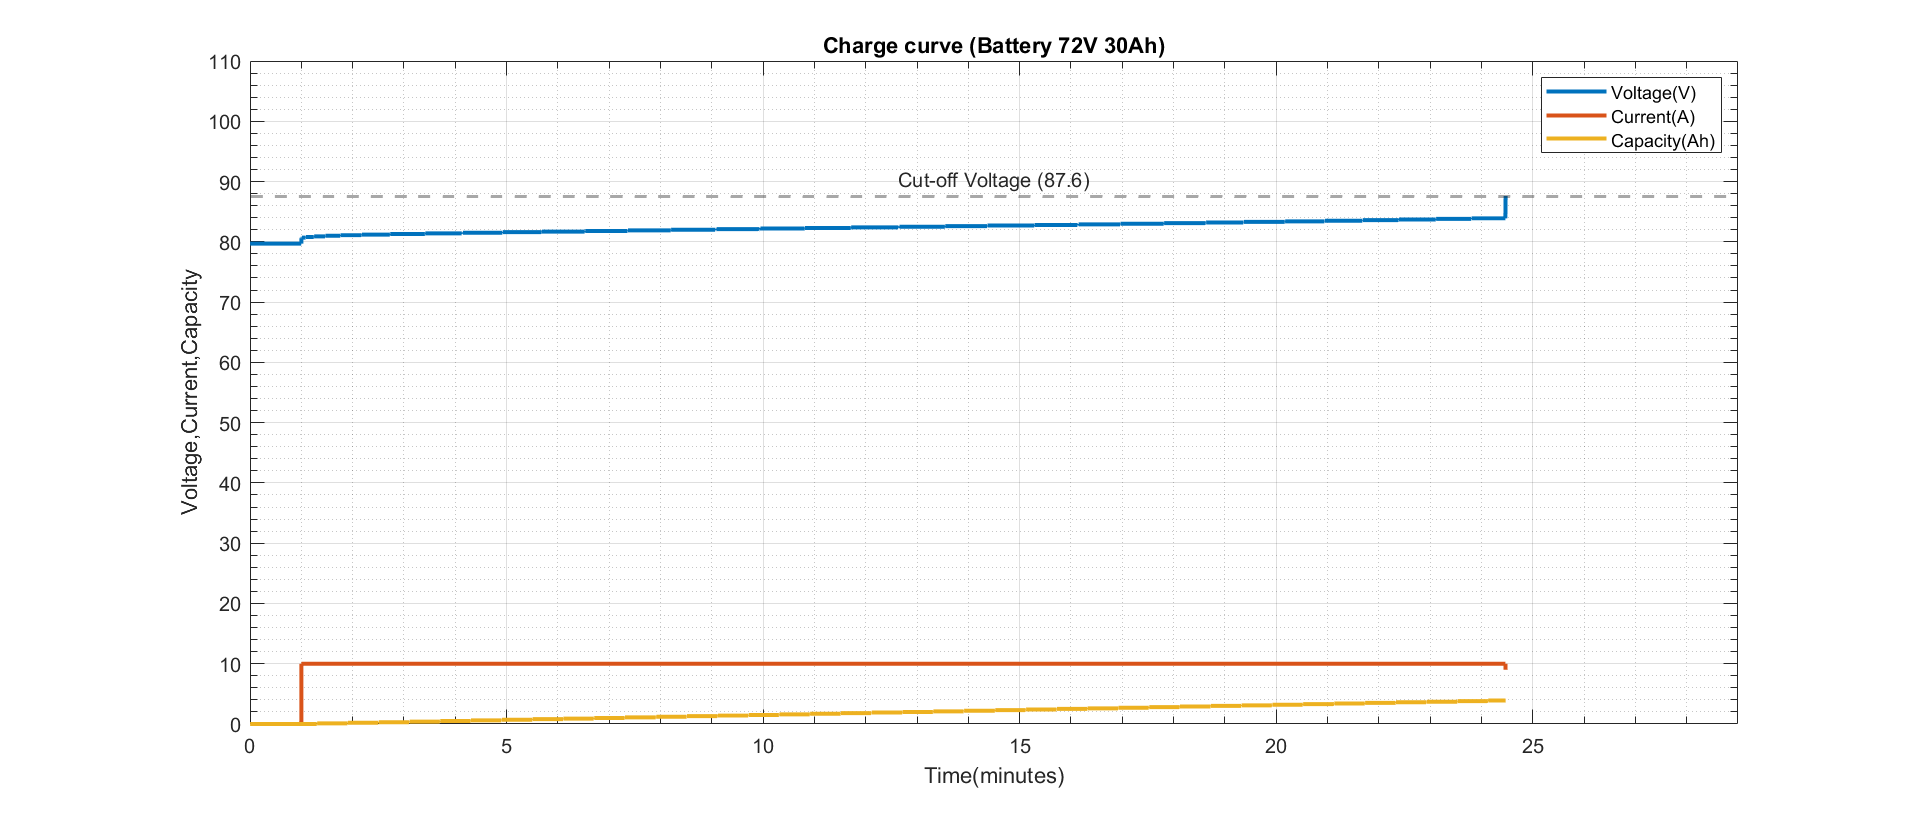
\includegraphics[width=\paperwidth]{Chapters/img/Result/Charge curve 72V30Ah_OV.png}}
		\centering
		\captionsetup{justification=centering,margin=2cm}
		\caption{กราฟการทดสอบการป้องกันการชาร์จเกินของแบตเตอรี่ 72V30Ah}
	\end{figure}
\end{center}
จากการทดสอบพบว่าแบตเตอรี่สำหรับจักรยานยนต์ไฟฟ้าในระหว่างการทดสอบไม่มีการรั่วไหลของ\\อิเล็กโทรไลต์ ไม่มีการแตกหักหรือฉีกขาด ไม่เกิดเพลิงไหม้ และไม่เกิดการระเบิด
โดยการทดสอบการชาร์จนี้ถูกขัดจังหวะโดยระบบการจัดการแบตเตอรี่(BMS)ของโมดูลแบตเตอรี่นี้เองโดยขัดจังหวะเมื่อแรงดันของโมดูลแบตเตอรี่อยู่ที่ 83.9V 
หลังจากที่หยุดการชาร์จจากนั้นผู้ทดสอบได้ทำการสังเกตแบตเตอรี่เป็นระยะเวลา 1 ชั่วโมงพบว่าแบตเตอรี่ยังคงสภาพปกติและยังคงสามารถใช้งานได้
\newline\hspace*{2cm}
ผลจากการทดสอบแบตเตอรี่สำหรับรถสามล้อไฟฟ้า 72V 60Ah มีดังนี้
\begin{center}
	\begin{figure}[H]
	\makebox[\textwidth]{
	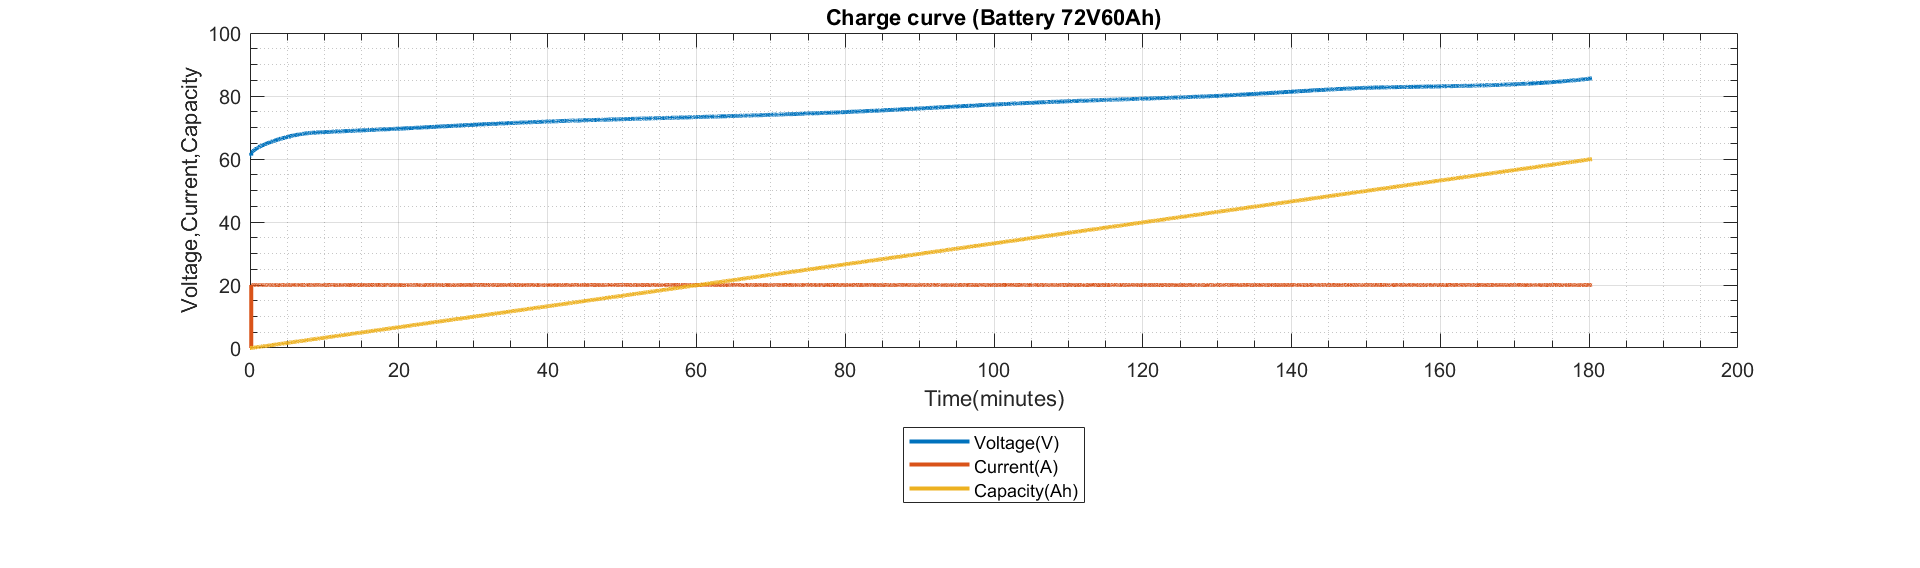
\includegraphics[width=\paperwidth]{Chapters/img/Result/Charge curve 72V60Ah.png}}
		\centering
		\captionsetup{justification=centering,margin=2cm}
		\caption{กราฟการทดสอบการป้องกันการชาร์จเกินของแบตเตอรี่ 72V60Ah}
	\end{figure}
\end{center}
จากการทดสอบพบว่าแบตเตอรี่สำหรับรถสามล้อไฟฟ้าระหว่างการทดสอบไม่มีการรั่วไหลของอิเล็กโทรไลต์ ไม่มีการแตกหักหรือฉีกขาด ไม่เกิดเพลิงไหม้ และไม่เกิดการระเบิด
แต่การทดสอบนั้นถูกขัดจังหวะโดยผู้ทดสอบเองโดยขัดจังหวะที่แรงดันของโมดูลแบตเตอรี่อยู่ที่ 85.6V เนื่องจากหากดำเนินการทดสอบต่อไปอาจจะทำให้เกิดความเสียหายกับแบตเตอรี่และอุปกรณ์การทดสอบได้ซึ่ง
หลังจากที่หยุดการชาร์จผู้ทดสอบได้ทำการสังเกตแบตเตอรี่เป็นระยะเวลา 1 ชั่วโมงพบว่าแบตเตอรี่ยังคงสภาพปกติและยังคงสามารถใช้งานได้
\newline\hspace*{2cm}
ผลจากการทดสอบแบตเตอรี่ 72V 72Ah มีดังนี้
\begin{center}
	\begin{figure}[H]
	\makebox[\textwidth]{
	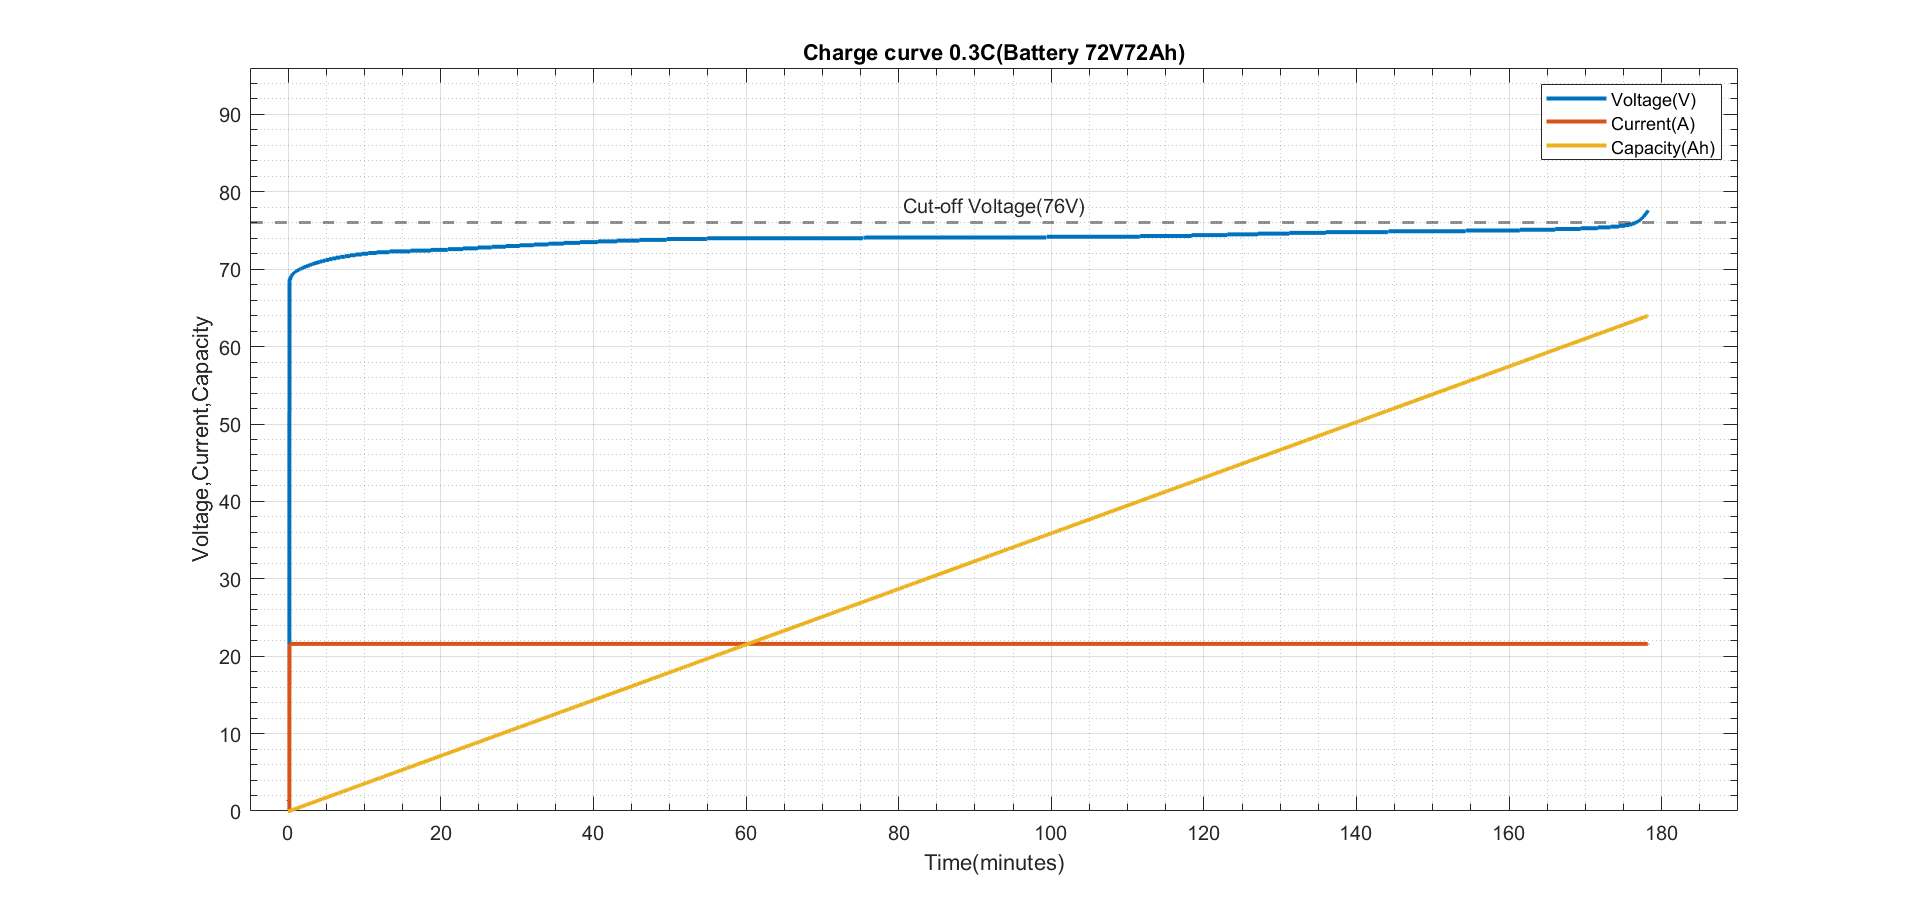
\includegraphics[width=\paperwidth]{Chapters/img/Result/Charge curve 0.3C 72V72Ah.png}}
		\centering
		\captionsetup{justification=centering,margin=2cm}
		\caption{กราฟการทดสอบการป้องกันการชาร์จเกินของแบตเตอรี่ 72V72Ah}
	\end{figure}
\end{center}
จากการทดสอบพบว่าแบตเตอรี่สำหรับรถสามล้อไฟฟ้าระหว่างการทดสอบไม่มีการรั่วไหลของอิเล็กโทรไลต์ ไม่มีการแตกหักหรือฉีกขาด ไม่เกิดเพลิงไหม้ และไม่เกิดการระเบิด
โดยการทดสอบการชาร์จนี้ถูกขัดจังหวะโดยระบบการจัดการแบตเตอรี่(BMS)ของโมดูลแบตเตอรี่นี้เองโดยขัดจังหวะเมื่อแรงดันของโมดูลแบตเตอรี่อยู่ที่ 77.6V 
หลังจากที่หยุดการชาร์จจากนั้นผู้ทดสอบได้ทำการสังเกตแบตเตอรี่เป็นระยะเวลา 1 ชั่วโมงพบว่าแบตเตอรี่ยังคงสภาพปกติและยังคงสามารถใช้งานได้
%----------------------------------------------------------------------------------
\subsection{ผลการทดสอบการป้องกันการดิสชาร์จเกิน}
สำหรับการทดสอบการป้องกันการดิสชาร์จเกินของแบตเตอรี่สำหรับจักรยานยนต์ไฟฟ้า 72V 30Ah มีดังนี้
\begin{center}
	\begin{figure}[H]
	\makebox[\textwidth]{
	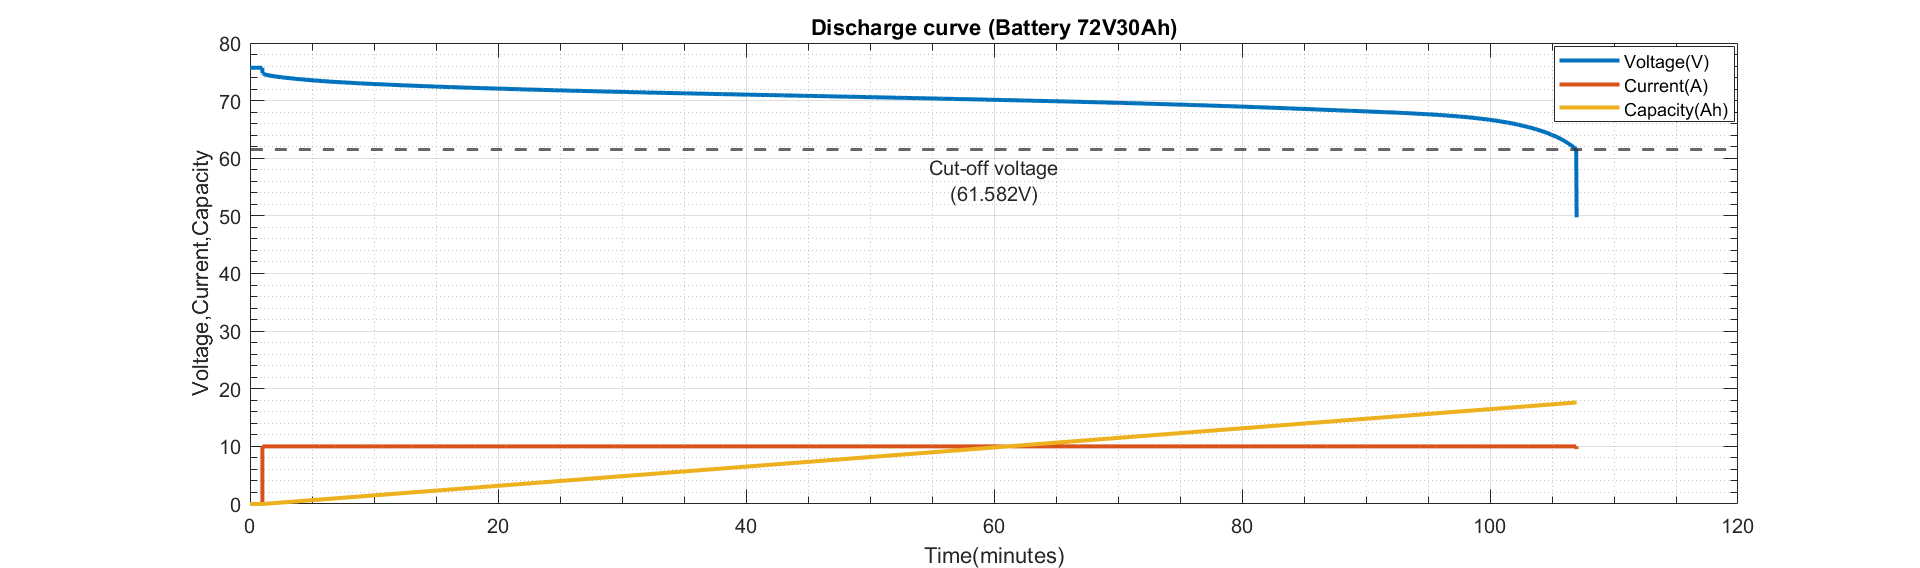
\includegraphics[width=\paperwidth]{Chapters/img/Result/Discharge curve 72V30Ah.png}}
		\centering
		\captionsetup{justification=centering,margin=2cm}
		\caption{กราฟการทดสอบการป้องกันการดิสชาร์จเกินของแบตเตอรี่ 72V30Ah}
	\end{figure}
\end{center}
จากการทดสอบพบว่าแบตเตอรี่สำหรับจักรยานยนต์ไฟฟ้าในระหว่างการทดสอบไม่มีการรั่วไหลของอิเล็กโทรไลต์ ไม่มีการแตกหักหรือฉีกขาด ไม่เกิดเพลิงไหม้ และไม่เกิดการระเบิด
โดยการทดสอบการดิสชาร์จนี้ถูกขัดจังหวะโดยระบบการจัดการแบตเตอรี่(BMS)ของโมดูลแบตเตอรี่นี้เองโดยขัดจังหวะเมื่อแรงดันของโมดูลแบตเตอรี่อยู่ที่ 61.582V 
หลังจากที่หยุดการชาร์จจากนั้นผู้ทดสอบได้ทำการสังเกตแบตเตอรี่เป็นระยะเวลา 1 ชั่วโมงพบว่าแบตเตอรี่ยังคงสภาพปกติและยังคงสามารถใช้งานได้
\newline\hspace*{2cm}
ผลจากการทดสอบแบตเตอรี่สำหรับรถสามล้อไฟฟ้า 72V 60Ah มีดังนี้
\begin{center}
	\begin{figure}[H]
	\makebox[\textwidth]{
	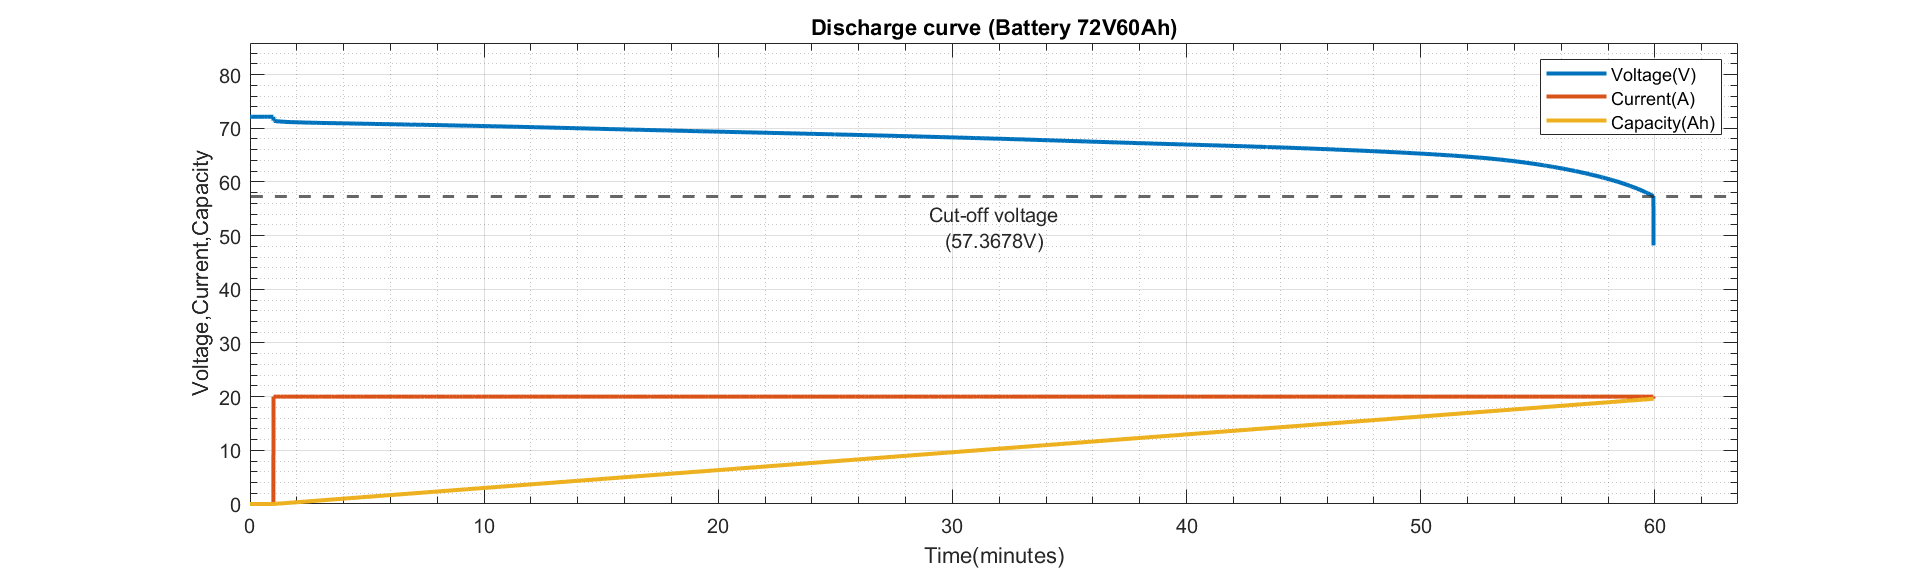
\includegraphics[width=\paperwidth]{Chapters/img/Result/Discharge curve 72V60Ah.png}}
		\centering
		\captionsetup{justification=centering,margin=2cm}
		\caption{กราฟการทดสอบการป้องกันการดิสชาร์จเกินของแบตเตอรี่ 72V60Ah}
	\end{figure}
\end{center}
\hspace*{2cm}
จากการทดสอบพบว่าแบตเตอรี่สำหรับรถสามล้อไฟฟ้าระหว่างการทดสอบไม่มีการรั่วไหลของอิเล็กโทรไลต์ ไม่มีการแตกหักหรือฉีกขาด ไม่เกิดเพลิงไหม้ และไม่เกิดการระเบิด
โดยการทดสอบการดิสชาร์จนี้ถูกขัดจังหวะโดยระบบการจัดการแบตเตอรี่(BMS)ของโมดูลแบตเตอรี่นี้เองโดยขัดจังหวะเมื่อแรงดันของโมดูลแบตเตอรี่อยู่ที่ 57.3678V 
หลังจากที่หยุดการชาร์จจากนั้นผู้ทดสอบได้ทำการสังเกตแบตเตอรี่เป็นระยะเวลา 1 ชั่วโมงพบว่าแบตเตอรี่ยังคงสภาพปกติและยังคงสามารถใช้งานได้
%=====================================================================================================
\newline\hspace*{2cm}
ผลจากการทดสอบแบตเตอรี่ 72V 72Ah มีดังนี้
\begin{center}
	\begin{figure}[H]
	\makebox[\textwidth]{
	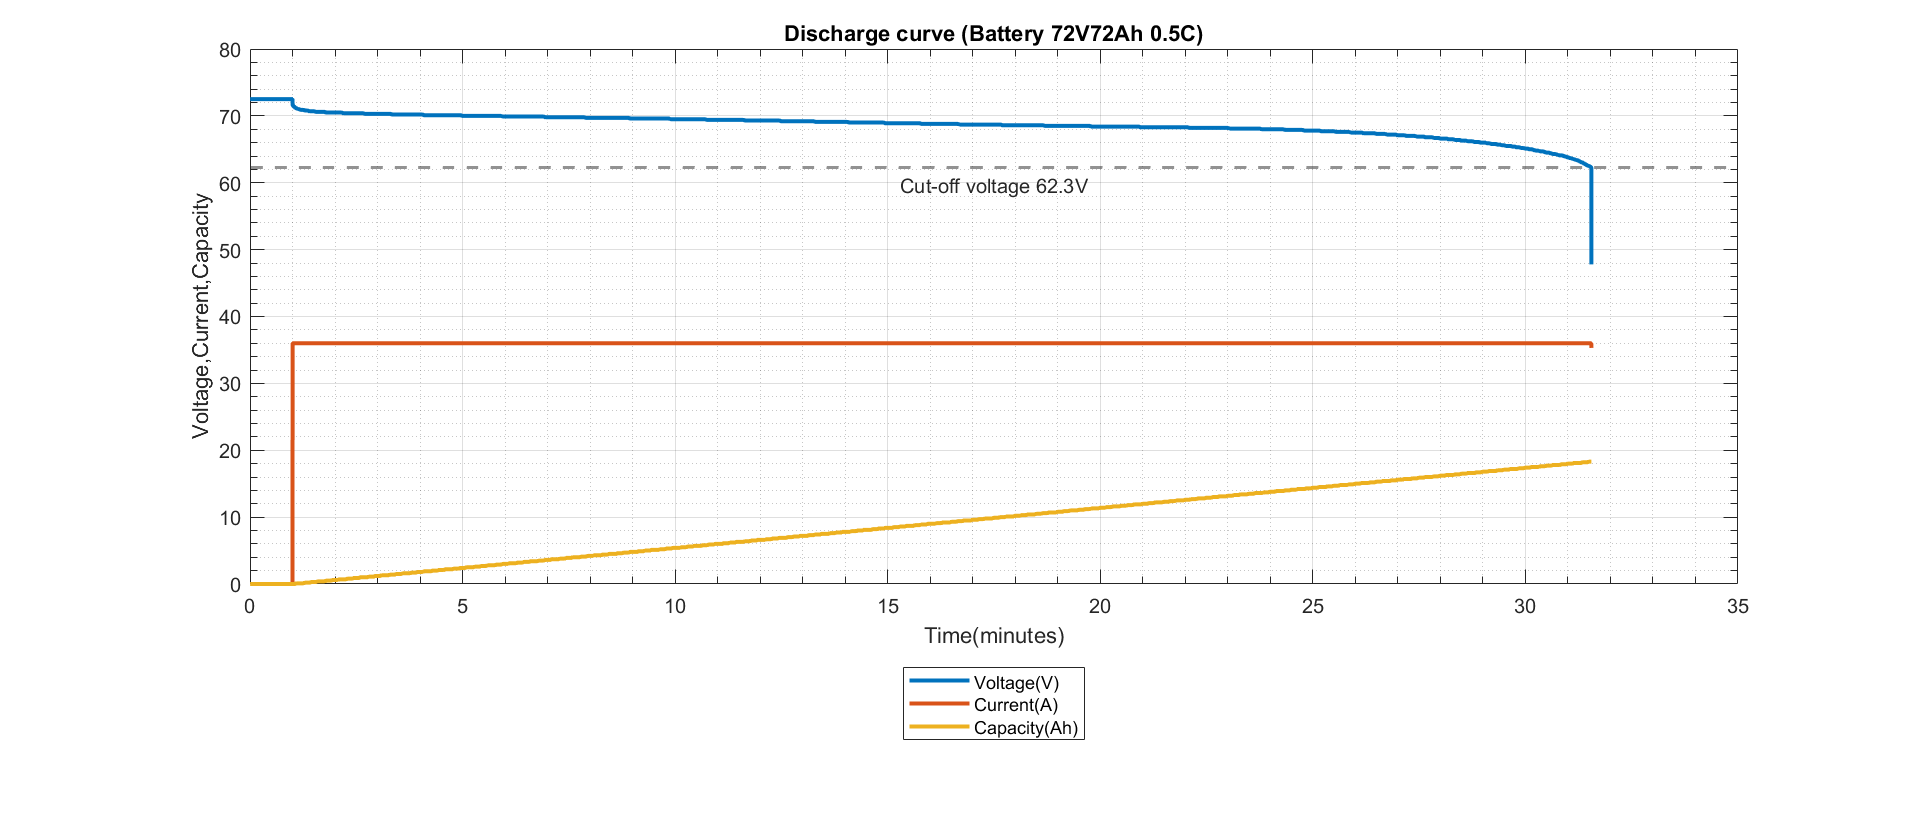
\includegraphics[width=\paperwidth]{Chapters/img/Result/Discharge curve 0.5C 72V72Ah.png}}
		\centering
		\captionsetup{justification=centering,margin=2cm}
		\caption{กราฟการทดสอบการป้องกันการดิสชาร์จเกินของแบตเตอรี่ 72V72Ah}
	\end{figure}
\end{center}
\hspace*{2cm}
จากการทดสอบพบว่าแบตเตอรี่สำหรับรถสามล้อไฟฟ้าระหว่างการทดสอบไม่มีการรั่วไหลของอิเล็กโทรไลต์ ไม่มีการแตกหักหรือฉีกขาด ไม่เกิดเพลิงไหม้ และไม่เกิดการระเบิด
โดยการทดสอบการดิสชาร์จนี้ถูกขัดจังหวะโดยระบบการจัดการแบตเตอรี่(BMS)ของโมดูลแบตเตอรี่นี้เองโดยขัดจังหวะเมื่อแรงดันของโมดูลแบตเตอรี่อยู่ที่ 62.3V 
หลังจากที่หยุดการชาร์จจากนั้นผู้ทดสอบได้ทำการสังเกตแบตเตอรี่เป็นระยะเวลา 1 ชั่วโมงพบว่าแบตเตอรี่ยังคงสภาพปกติและยังคงสามารถใช้งานได้
%=====================================================================================================
\section{ผลการทดสอบอื่นๆ}
\subsection{ผลการทดสอบการวัดความต้านทานภายในของแบตเตอรี่}
จากรูป\ref{fig:DCIR_Test}ซึ่งเป็นกราฟการทดสอบการวัดความต้านทานภายในของโมดูลแบตเตอรี่ 72V72Ah ซึ่งทดสอบขณะที่โมดูลแบตเตอรี่มีแรงดันขณะสภาวะไม่มีโหลดที่ 72V และเริ่มทดสอบด้วยการ
ดิสชาร์จที่อัตรากระแส 0.2C เป็นระยะเวลา 10 วินาทีและจากนั้นจึงดิสชาร์จด้วยอัตรากระแส 1C เป็นระยะเวลา 1 วินาทีโดยผลการทดสอบนี้ทำให้ได้ค่าความต้านทานภายในของแบตเตอรี่โมดูลนี้อยู่ที่ $26.8m\Omega$
\begin{center}
	\begin{figure}[H]
	\makebox[\textwidth]{
	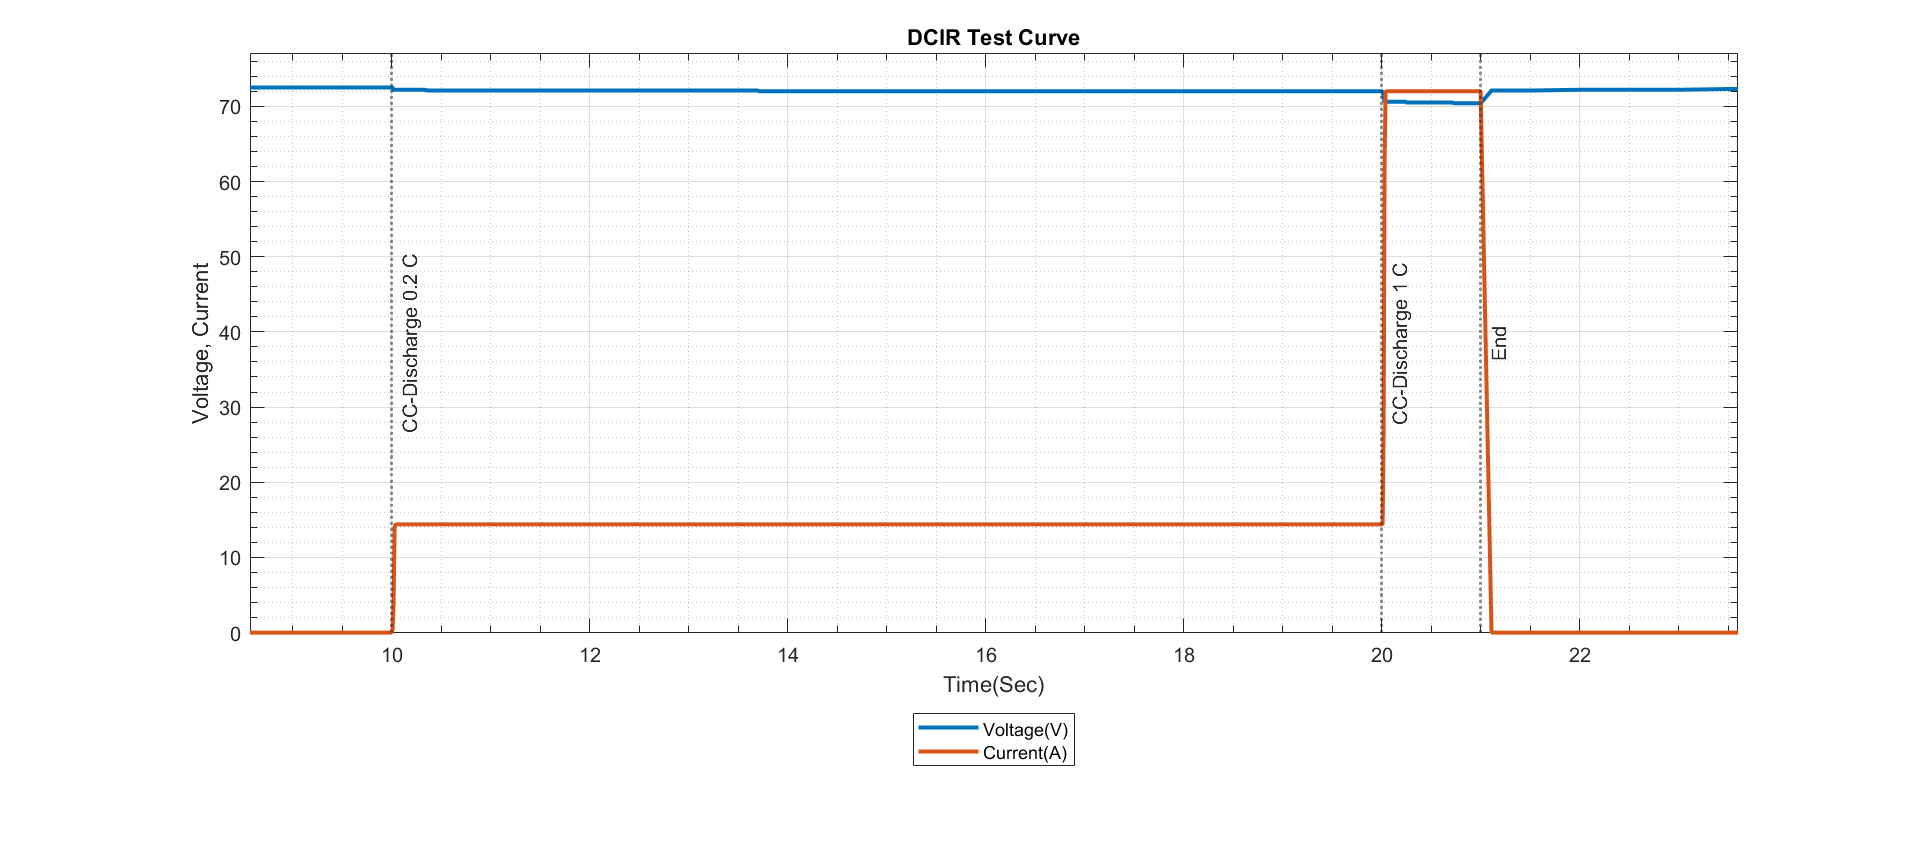
\includegraphics[width=\paperwidth]{Chapters/img/Result/DCIR_TEST.png}}
		\centering
		\captionsetup{justification=centering,margin=2cm}
		\caption{กราฟการทดสอบการวัดความต้านทานภายในของแบตเตอรี่ 72V72Ah}
		\label{fig:DCIR_Test}
	\end{figure}
\end{center}
%----------------------------------------------------------------------------------
\pagebreak
\subsection{ผลการทดสอบระยะเวลาในการพักของแบตเตอรี่}
จากรูป\ref{fig:Rest_Test} การทดสอบนี้หลังจากการดิสชาร์จที่กระแส 0.5C โดยหลังจากการดิสชาร์จแล้วแรงดันของโมดูลแบตเตอรี่จะเพิ่มขึ้นทีละน้อยเมื่อระยะเวลาผ่านไปโดยประมาณ 30 นาที
แรงดันจึงไม่เกิดการเปลี่ยนแปลง
\begin{center}
	\begin{figure}[H]
	\makebox[\textwidth]{
	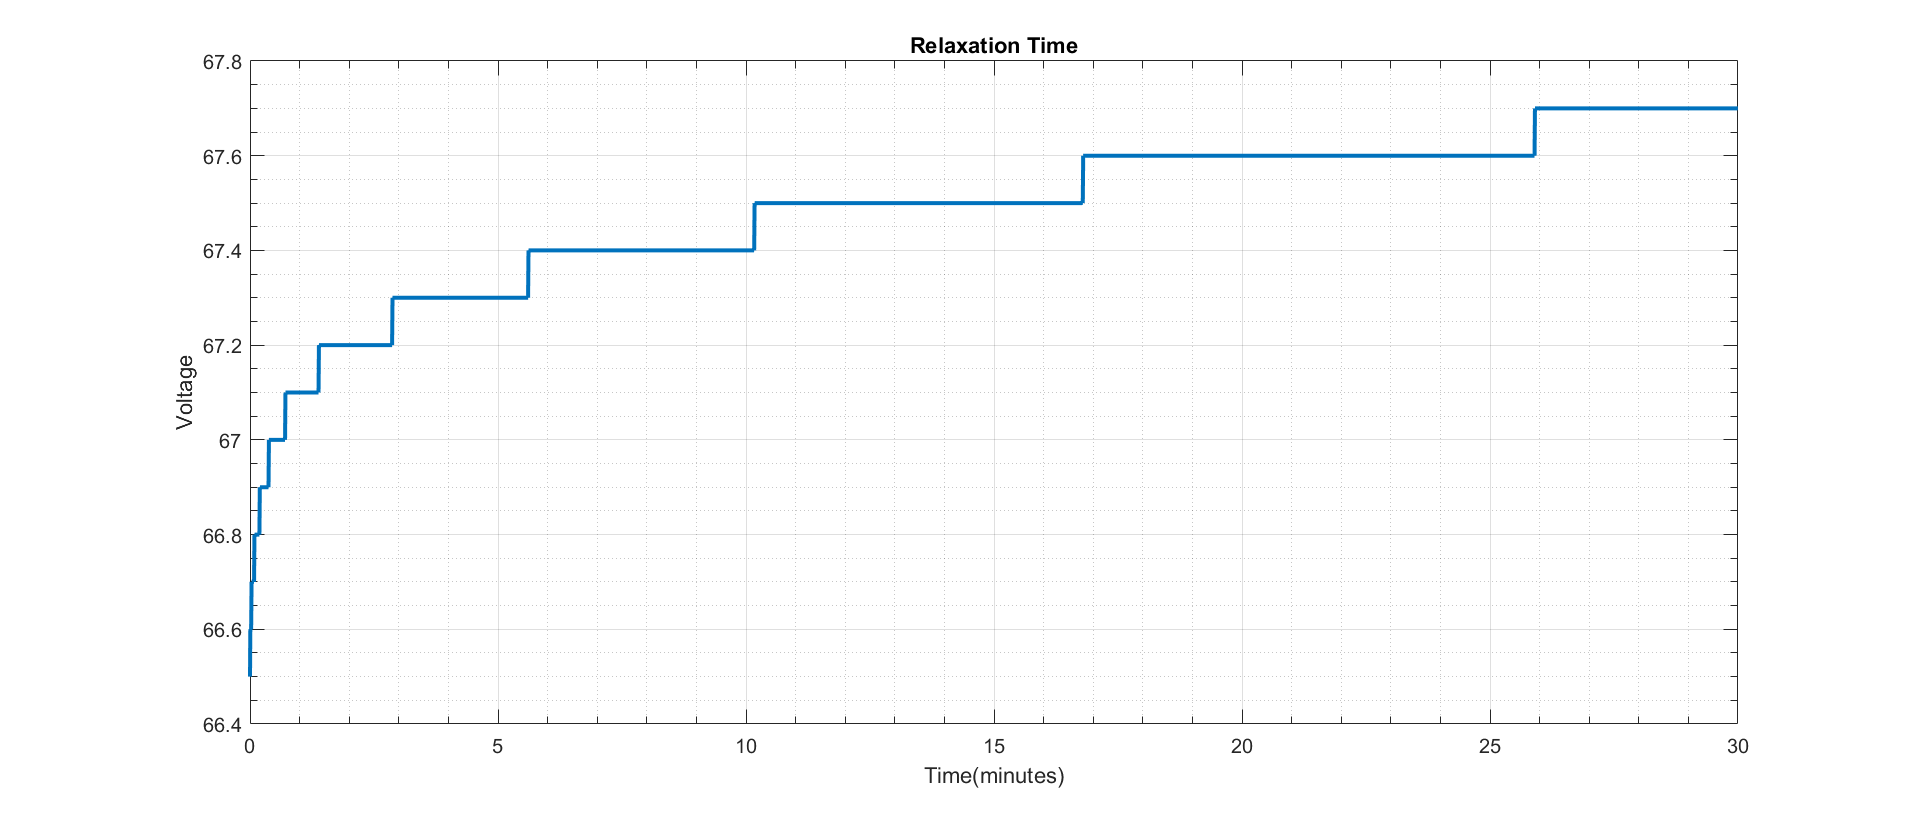
\includegraphics[width=\paperwidth]{Chapters/img/Result/Relaxation Time.png}}
		\centering
		\captionsetup{justification=centering,margin=2cm}
		\caption{กราฟการทดสอบระยะเวลาพักแบตเตอรี่ 72V72Ah}
		\label{fig:Rest_Test}
	\end{figure}
\end{center}
%----------------------------------------------------------------------------------
\pagebreak
\subsection{ผลการทดสอบอัตรากระแส}
จากรูป\ref{fig:C_rate_Test} การทดสอบอัตรากระแสนี้ได้จากการทดสอบดิสชาร์จแบตเตอรี่ 72V72Ah ด้วยอัตรากระแส 0.3C เทียบกับอัตรากระแส 0.5C ซึ่งจะเห็นได้ว่าและความจุจากการที่ดิสชาร์จ
ด้วยอัตรากระแสที่มากกว่าทำให้แรงดันนั้นลดลงรวดเร็วมากกว่าการดิสชาร์จด้วยอัตรากระแสที่น้อยกว่าเช่นเดียวกับความจุที่ลดลงอย่างรวดเร็วเช่นเดียวกันซึ่งขณะที่ทดสอบแบตเตอรี่มีแรงดันอยู่ที่ 72V
\begin{center}
	\begin{figure}[H]
	\makebox[\textwidth]{
	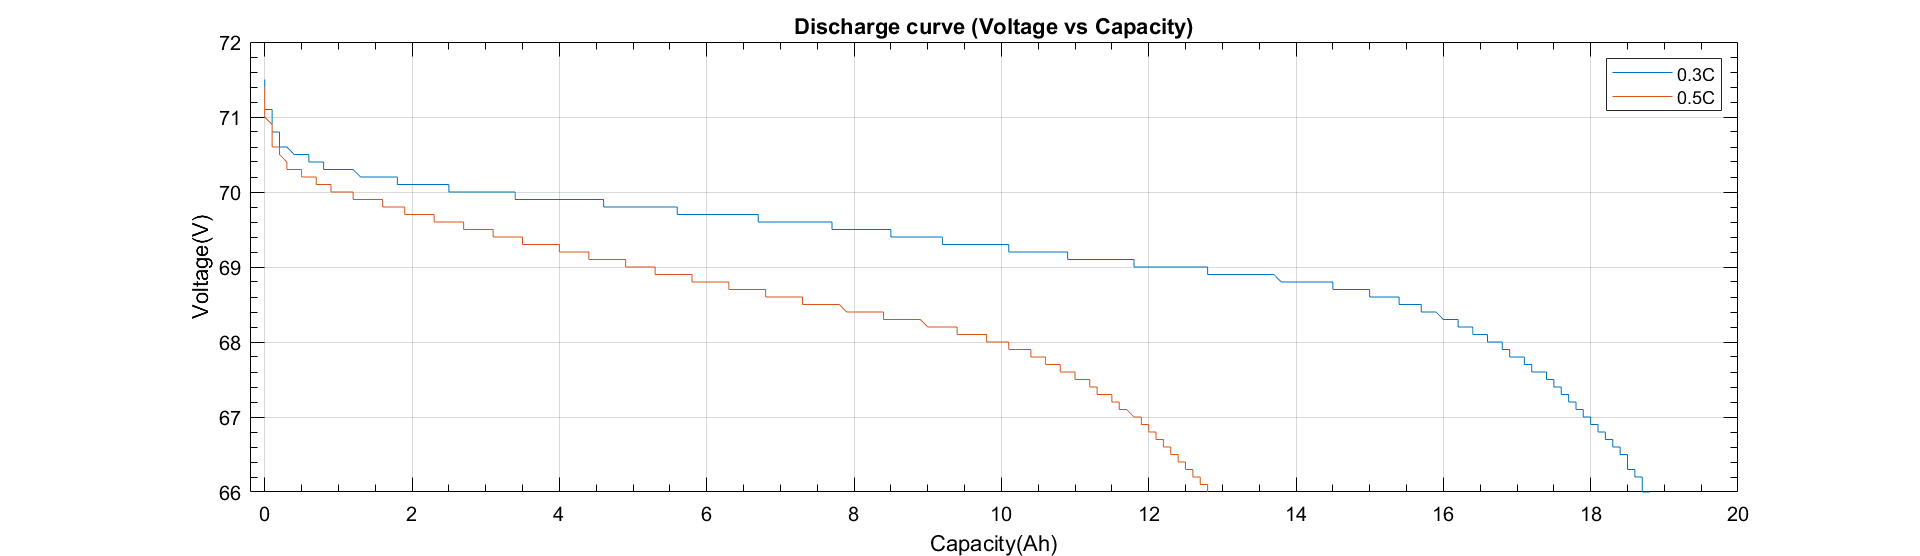
\includegraphics[width=\paperwidth]{Chapters/img/Result/Discharge curve V vs Ah.png}}
		\centering
		\captionsetup{justification=centering,margin=2cm}
		\caption{กราฟการทดสอบอัตรากระแสดิสชาร์จ 72V72Ah}
		\label{fig:C_rate_Test}
	\end{figure}
\end{center}